% arara: pdflatex: {synctex: yes, action: batchmode, draft: yes, options: "-halt-on-error -file-line-error-style"}
% arara: bibtex
% arara: pdflatex: {synctex: yes, action: batchmode, draft: yes, options: "-halt-on-error -file-line-error-style"}
% arara: pdflatex: {synctex: yes, action: nonstopmode, options: "-halt-on-error -file-line-error-style"}

%%% Preamble
\documentclass[ DIV=calc,%
                paper=a4,%
                fontsize=12pt,%
                twocolumn%
              ]{scrartcl}	 			% KOMA-article class

\usepackage[utf8]{inputenc}
\usepackage{lipsum}												% Package to create dummy text

\usepackage[english]{babel}										% English language/hyphenation
\usepackage[protrusion=true,expansion=true]{microtype}			% Better typography
\usepackage{amsmath,amsfonts,amsthm}					        % Math packages
\usepackage[pdftex]{graphicx}			                        % Enable pdflatex
\usepackage[svgnames]{xcolor}			                        % Enabling colors by their 'svgnames'
\usepackage[hang, small,labelfont=bf,up,textfont=it,up]{caption} % Custom captions under/above floats
\usepackage{epstopdf}											% Converts .eps to .pdf
\usepackage{subfig}												% Subfigures
\usepackage{booktabs}											% Nicer tables
\usepackage{fix-cm}												% Custom fontsizes


%%% Custom sectioning (sectsty package)
\usepackage{sectsty}							% Custom sectioning (see below)
\allsectionsfont{%								% Change font of al section commands
	\usefont{OT1}{phv}{b}{n}%					% bch-b-n: CharterBT-Bold font
	}

\sectionfont{%									% Change font of \section command
	\usefont{OT1}{phv}{b}{n}%					% bch-b-n: CharterBT-Bold font
	}


%%% Headers and footers
\usepackage{fancyhdr}						    % Needed to define custom headers/footers
	\pagestyle{fancy}							% Enabling the custom headers/footers
\usepackage{lastpage}	



%%% Title, author and date metadata
\newcommand{\Title}{BitTorrent on a diet}
\newcommand{\Subtitle}{Peer-to-peer file distribution in wireless sensor networks}
\newcommand{\Author}{Mattias Buelens}
\newcommand{\Institute}{KU Leuven}
\newcommand{\Date}{February 2015}


\usepackage{titling}									% For custom titles

\newcommand{\HorRule}{\color{DarkBlue}%			% Creating a horizontal rule
									  	\rule{\linewidth}{1pt}%
										}

\pretitle{\vspace{-30pt} \begin{flushleft} \HorRule 
				\fontsize{50}{50} \usefont{OT1}{phv}{b}{n} \color{DarkBlue} \selectfont 
				}
\title{\Title}
\posttitle{
                    \par\vskip 0.5em \fontsize{30}{30} \selectfont \Subtitle
                    \par\end{flushleft}\vskip 0.5em}

\preauthor{\begin{flushleft}
					\large \lineskip 0.5em \usefont{OT1}{phv}{b}{sl} \color{DarkBlue}}
\author{\Author, }
\postauthor{\footnotesize \usefont{OT1}{phv}{m}{sl} \color{Black} 
					\Institute
					\par\end{flushleft}\HorRule}
%\date{\Date}
\date{}

% Header (empty)
\lhead{}
\chead{}
\rhead{}
% Footer (you may change this to your own needs)
\lfoot{\footnotesize \textbf{\Author} \textbullet ~ \Title: \Subtitle}
\cfoot{}
\rfoot{\footnotesize page \thepage\ of \pageref{LastPage}}	% "page 1 of 2"
\renewcommand{\headrulewidth}{0.0pt}
\renewcommand{\footrulewidth}{0.4pt}

% Columns
\setlength{\columnsep}{0.5cm}
%\setlength{\columnseprule}{0.75pt}


%%% Begin document
\begin{document}
\maketitle
\thispagestyle{fancy} 			% Enabling the custom headers/footers for the first page
\textbf{The internet is in everything. Just a few decades ago, you had to sit in front of a big clunky machine on your desktop and dial in through a sluggish 56k modem to connect to the internet. Today, you can surf the web on your laptop, your mobile phone, your TV and even your wristwatch. And the invasion of the internet doesn't stop there. In the future, the ``internet of things'' will connect many small battery-powered devices to work together and help monitor and control an environment.}

\textbf{However, how do you keep the software on these devices up-to-date without wasting too much battery and reducing their lifespan? \Author, an engineering master student from \Institute{} university, is working on a thesis to design an implement a protocol which can serve such software updates fast and efficiently by taking some ideas from the peer-to-peer file transfer protocol BitTorrent.}

\vfill\eject

\section*{Context}
In the ``internet of things'', everything from your washing machine to your central heating system will have an internet connection so you can monitor and control them from everywhere. These small embedded devices communicate with you and with each other in a so-called ``wireless sensor network'' (WSN) to measure and react upon their environment. They can be tasked with anything from simply keeping your house warm during the winter, to monitoring an active volcano and alerting for possible eruptions as shown in figure \ref{fig:reventador}.

These embedded devices are installed with a sufficient battery and a wireless connection to do their job for many years without interruption. Often, it is impractical or impossible to manually fix such a device after its installation. For example, these devices may be embedded in a thick wall, or may be dropped near the crater of a volcano. When a bug in the initial software is discovered or a new feature is developed, it is necessary that the updated software can be deployed without physical access to the device. Using their wireless connection, these devices can receive an `over-the-air' update to their configuration or software to keep them running for many more years to come.

However, such wireless software deployments eat up quite a bit of battery juice, which can reduce the lifespan of the device. When all devices naively start to download a new software version from one single source, the nodes closest to the source will have to route a lot of data from the source to many distant nodes in the network. This large amount of network traffic going through a few nodes causes these nodes to use up more energy and therefore reduce their lifespan more quickly than more distant nodes. This load imbalance is bad for the whole network: if the nodes close to the source fail sooner, the rest of the network could become disconnected from the source. Moreover, most of the generated traffic is redundant, since the same file passes multiple times over some nodes in the network to be routed to distant nodes (figure \ref{fig:ftp_traffic}).

Therefore, a smarter deployment protocol is needed which better balances the load over all devices, utilizes the knowledge about the file at other nodes to reduce redundant traffic, but still deploys the software reasonably fast to every node in the network.

\begin{figure}
    \centering
    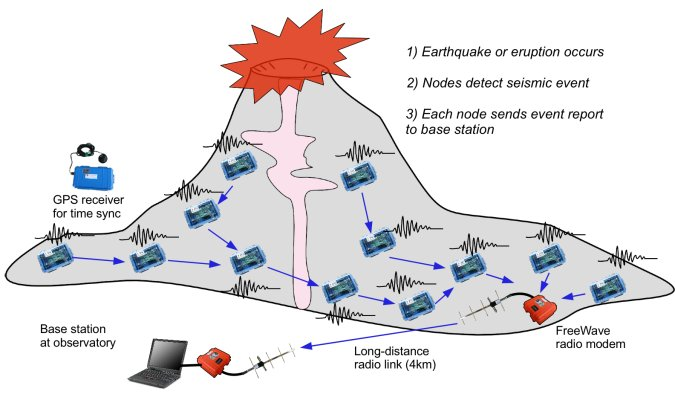
\includegraphics[width=\columnwidth]{images/reventador.jpg}
    \caption{A wireless sensor network deployed by the Harvard Sensor Networks Lab on an active volcano to monitor seismic activity. \cite{reventador}}
    \label{fig:reventador}
\end{figure}

\begin{figure}
    \centering
    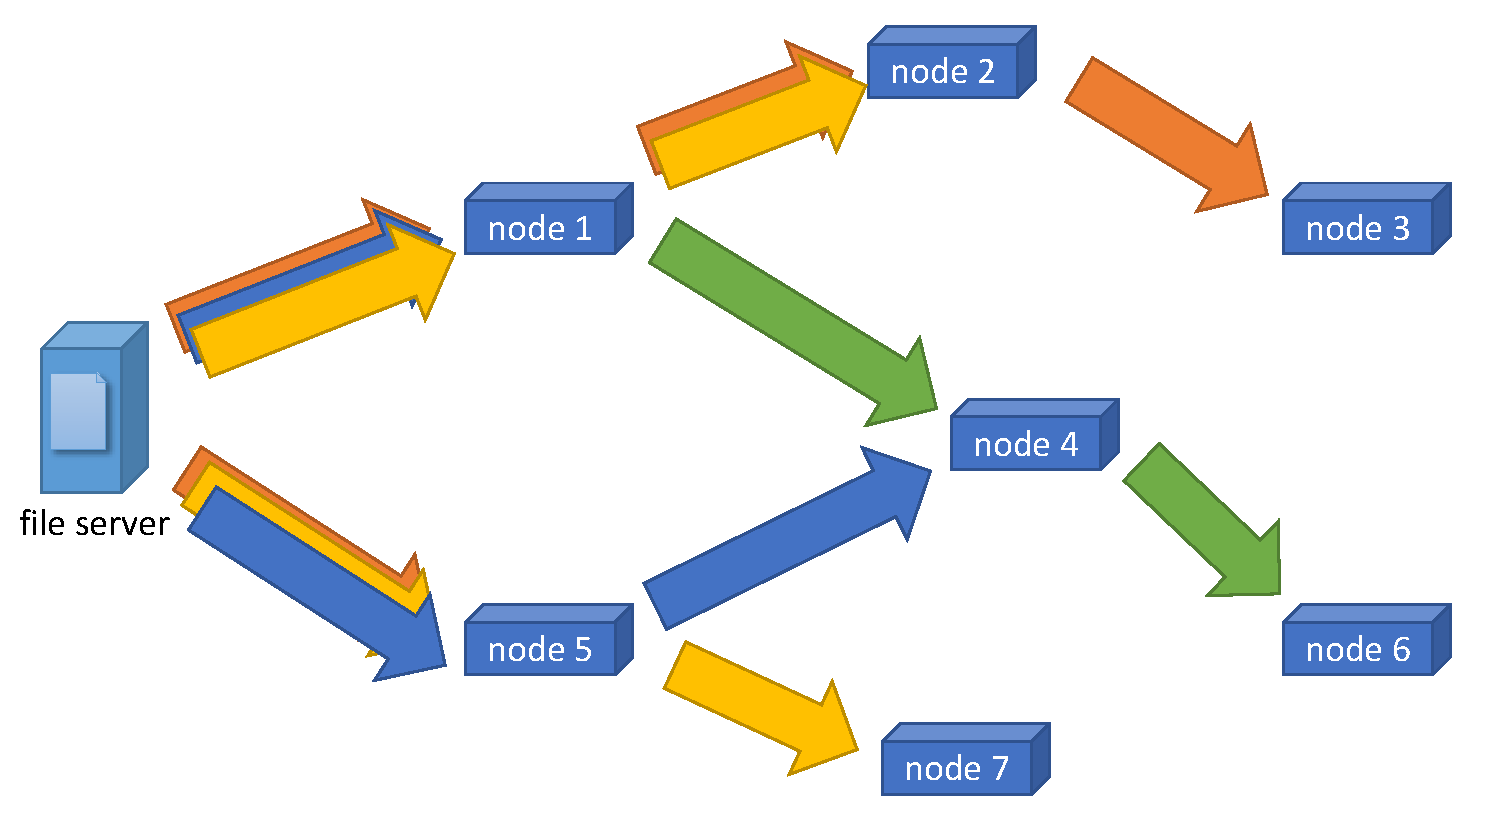
\includegraphics[width=\columnwidth]{diagrams/ftp_diagram.pdf}
    \caption{Illustration of network traffic generated by a naive file distribution protocol. The file server needs to send the complete file over different separate connections to every node in the network. This leads to a lot of redundant traffic passing through the nodes closer to the server.}
    \label{fig:ftp_traffic}
\end{figure}

\section*{Inspiration from BitTorrent}
\subsection*{What is BitTorrent?}
Many people have already heard about or even used BitTorrent to download large files on the internet, such as movies, games or complete Linux distributions. However, few know what it actually is or how it works.

In essence, BitTorrent is a peer-to-peer file transfer protocol: instead of downloading a file from one single source (server), you download pieces of the file from other people who already downloaded that piece for themselves. Your computer becomes a `peer' in the torrent's `swarm', and starts downloading pieces from other peers but also uploading your downloaded pieces to others.

This allows others to benefit from your upload capacity, which would otherwise be unused by a standard client-server protocol such as FTP. This is one of the original design goals of BitTorrent, and manifests itself clearly in the internet statistics where it is responsible for 25\% of the world's upload traffic \cite{sandvine}.

In order to join the swarm, BitTorrent uses a centralized tracker which is responsible for keeping track of the swarm. A new peer first contacts the tracker, which replies with a list of peers to connect with. From then on, the peer can connect with (some of) these other peers and start downloading pieces. When a peer wants to leave the swarm, it also announces this to the tracker so it will no longer advertise it to other peers. Although the tracker is a centralized entity and thus a potential single point of failure, the file transfer itself is fully decentralized. This means that the tracker only needs to store the torrent's information and the list of all peers in the swarm, and doesn't need to know the actual contents of the file being distributed.

This is especially interesting for content providers who want to serve large files to many clients. Instead of putting the full load of the file distribution on a single server, BitTorrent can share the load over every peer in the swarm. As long as every piece of the file is available from at least one peer in the swarm, every peer can receive the whole file. A content provider therefore doesn't need to install a very powerful server to handle thousands of concurrent downloads: it only needs to keep one server in the swarm as the `initial seed' with the whole file, and the load is shared as soon as other peers download some pieces from the seed. When \emph{more} peers are downloading the file, the load on the initial seed actually \emph{decreases} as opposed to increasing in the case of classical server-client protocols.

\subsection*{Why BitTorrent in a WSN?}
Although BitTorrent was designed for file distribution across the whole internet, its ideas can be very useful for solving design challenges for our protocol.

BitTorrent provides load balancing over the peers in the swarm, which is especially interesting for wireless sensor networks. Instead of having every node download from a single server and generating a lot of traffic for the nodes near that server, the traffic can be more scattered over the whole network. Ideally, every node downloads and uploads about the same amount, draining every node's battery equally.

It is also fairly resilient to individual failures. When a peer leaves the swarm or crashes, the other peers can still communicate and continue downloading. When the peer rejoins the swarm later, it knows which pieces it had already downloaded and resume downloading the remaining pieces. This is useful for BitTorrent when downloading very large files in multiple sessions over many hours or even days, where having to restart the download after an interruption can mean a lot of wasted time. For a wireless sensor network deployed in a harsh environment, this kind of fault tolerance and recovery can allow for longer lifetime of the network.

\section*{Optimizations for WSNs}
Although BitTorrent is a good reference to start designing a peer-to-peer file transfer protocol, it cannot be used as-is for use in a wireless sensor network. WSNs are structured differently than the internet, nodes in a WSN are not as powerful as consumer computers, and battery consumption needs to be taken into account. This leads to optimizations in the protocol design targeted for WSNs.

\subsection*{Simple tracker for pairing up nodes}
The designed protocol uses a tracker much like BitTorrent's version, although in a slimmed down form. BitTorrent uses HTTP for its tracker communication and adds a lot of metadata for statistical purposes to the tracker messages (such as how much the peer has already uploaded or downloaded), which is not needed for the purposes of a wireless sensor network. Instead, the tracker communicates over UDP in small, structured messages and only keeps track of the list of peers in the swarm of a torrent.

\subsection*{Smaller files and pieces}
BitTorrent is used mostly for distributing very large files, often many GB in size. It splits up the file in fairly large pieces, usually a couple of MB per piece. A wireless sensor node only has a couple of KB of space, so the maximum file size and piece size for the designed protocol is very different. The protocol is designed for distributing small files around 2 to 4 KB in size, such as executable programs, configuration files or stored sensor measurements. These files can then be split up and distributed in pieces of around 256 bytes.

\subsection*{Local peers for reduced routing}
In order to achieve high download speed, it is important that you select peers which can provide a high upload speed \emph{to you}. This doesn't mean that everyone will get a high upload speed from a peer, the actual speed also depends on how close you are to that peer. A computer in Japan might have an upload bandwidth of 10 MB/s, but if the network between you and that Japanese peer is poor, you might only get 100 KB/s download speed on your end. On the other hand, your neighbour's computer uploading at 1 MB/s can probably provide you with a much better download speed, although it won't be able to serve other Japanese peers very well.

BitTorrent clients achieve this by monitoring the upload and download speed of each peer they're connected with, and then downloading from the peer which provides the best upload speed for you. This involves a lot of bookkeeping, and needs carefully considered strategies to work. These strategies also take into account punishing peers when they download a lot but do not upload in response (`leeching'), in order to discourage this unfair behaviour.

For wireless sensor networks, fairness is less of an issue: we assume that all nodes run the same protocol implementation and will not attempt to leech from others. Therefore, a simpler mechanism is employed: peers select a number of neighbouring peers, and also a few (two or three, depending on network size) remote peers which are farther away. They should then be able to download most of the file from their neighbours at high speeds, and receive missing pieces from the remote peers. In the worst case, a piece may be missing on both the neighbouring peers as well as the remote peers, in which case the peer needs to connect with a different remote peer (and optionally contact the tracker). This mechanism should allow for less negotiation overhead, while still providing decent piece availability and fairly high download speeds.

\section*{Future work}
Although the protocol design is sufficiently complete for a first implementation, it is far from being finalized.

For example, the protocol does not yet take the battery consumption of a node into account. It is possible that two peers both have a particular piece available, but their neighbouring peers all pick the same peer to download the piece from. This means that one peer has to send a lot of data, while the other is left underused. One possible solution would be to let peers keep track of their uploaded and downloaded amounts, and regularly announce these amounts with their neighbouring peers. The neighbours could then use this information to make a better selection of the peer to download from, and pick a less strained peer over an overworked one.

Experiments will be performed to analyze the impact on battery consumption to find out what improvements are worth implementing in the protocol.

\iffalse
\begin{figure}[b!]
    \centering
    \includegraphics[width=\textwidth,height=0.35\textheight,keepaspectratio]{network.jpg}
\end{figure}
\fi

%\vfill\eject

\section*{Conclusion}
Wireless sensor nodes in the ``internet of things'' need their software updates delivered fast but energy efficient. Therefore, a new protocol is being designed to distribute files on such nodes in a peer-to-peer fashion. The protocol is inspired by the popular BitTorrent file transfer protocol, but optimizes for wireless sensor networks by using smaller file and piece sizes and by relying on locality for high download speeds. With the major design decisions for the protocol complete, the protocol will now be further developed, implemented and tested on real wireless sensor nodes.

The major benchmark for the protocol will be if it indeed performs better than standard client-server file transfers, and in what circumstances. Intuitively, a client-server approach will have less overhead in a very small network where all nodes can directly reach the server. For larger networks, the peer-to-peer approach should theoretically perform better, but it will need more communication for bookkeeping purposes. Experiments will have to decide how much overhead is created in various configurations and if this indeed improves over the client-server approach.

In June 2015, you'll hopefully get an answer from \Author{} when he presents his master's thesis.

\clearpage
\onecolumn

\begin{flushleft}
\bibliographystyle{plain}
\bibliography{references-popular}
\end{flushleft}

\end{document}